\documentclass[../thesis.tex]{subfiles}

\begin{document}
\vspace{-1\baselineskip}

\section{The Large Hadron Collider}
\label{sec:LHC}
Predictions from theoretical models are evaluated against experimental data collected from particle detectors. This chapter provides a detailed overview of the Large Hadron Collider (\acs{LHC}) and the \acs{ATLAS} detector, one of the key experiments designed to study high-energy collisions at the \acs{LHC}.

\subsection{Overview}
The Large Hadron Collider \citep{Evans:2008zzb} (\acs{LHC}) is currently the world's largest particle collider with a circumference of almost 27 km. Built by \acs{CERN} on the border of Switzerland and France, the \acs{LHC} is designed as a particle collider for proton-proton (\acs{pp}), sometimes heavy ions i.e. lead-lead (PbPb) and proton-lead ($p$Pb) beams at TeV-scale energies. Two beams of particles are injected into the \acs{LHC} in opposite directions and allowed to collide at the center of four major experiments:
\begin{itemize}
\item \textbf{A Toroidal LHC ApparatuS} (\acs{ATLAS}) \citep{atlas} and \textbf{Compact Muon Solenoid} (\acs{CMS}) \citep{cms}: multi-purpose detectors, designed to target a variety of phenomena including \acs{SM}, \acs{BSM} and heavy-ion physics.
\item \textbf{Large Ion Collider Experiment} (\acs{ALICE}) \citep{alice}: specialized detector to record ion collisions and study heavy-ion physics.
\item \textbf{Large Hadron Collider beauty} (\acs{LHCb}) \citep{lhcb}: detector dedicated to study properties of $b$-quarks and $b$-hadrons.
\end{itemize}

Aside from the four major experiments, the \acs{LHC} also houses smaller experiments e.g. \acs{AWAKE} \citep{awake}, \acs{FASER} \citep{faser}, \acs{KATRIN} \citep{katrin}, that either share an interaction point with one of the above experiments or make use of particle beams pre-\acs{LHC} injection.

%\begin{wrapfigure}{r}{0.48\textwidth}
\begin{figure}[!htb]
\begin{center}
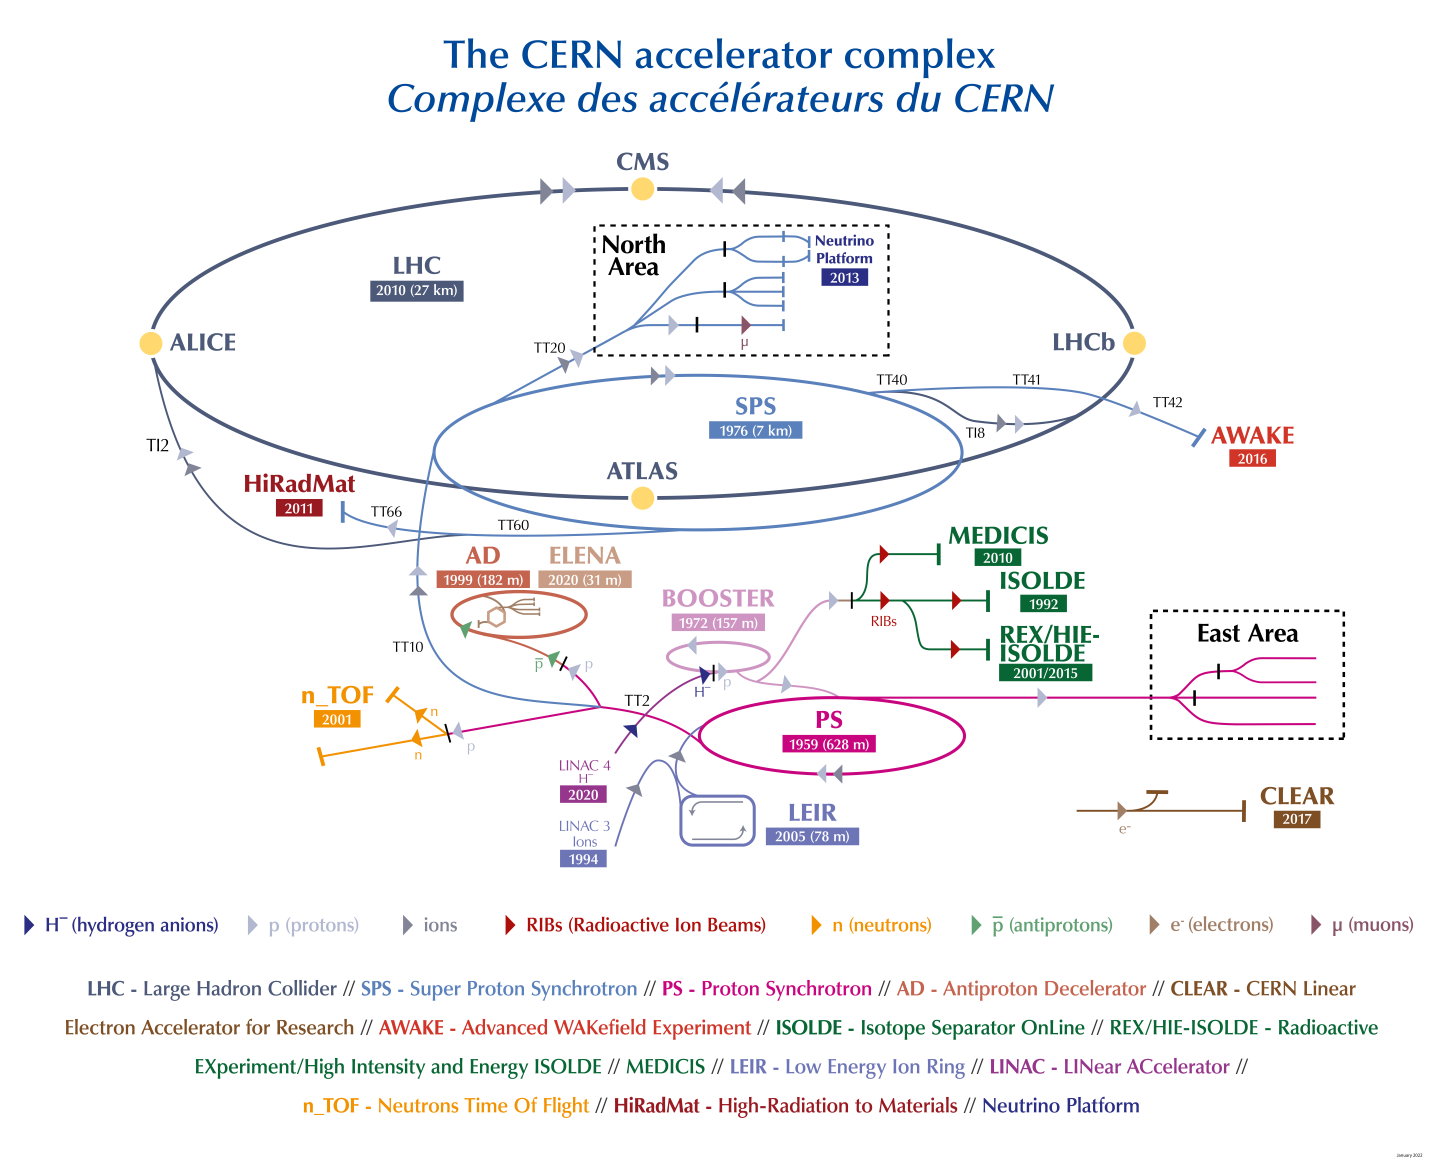
\includegraphics[width=\linewidth]{fig/lhc_map.png}
\caption[The full CERN accelerator complex as of 2022.]{\label{fig:lhc:map}The full \acs{CERN} accelerator complex as of 2022 \citep{fig:lhc_map}.}
\end{center}
\end{figure}
%\end{wrapfigure}

The majority of the \acs{LHC} operational time is dedicated to studying \acs{pp} collisions of up to $\sim$13 TeV center-of-mass energy, denoted as \acs{Ecom}. Reaching collision energy requires a sequence of accelerators within the \acs{CERN} accelerator complex, shown in \autoref{fig:lhc:map}. Proton production starts at \acs{LINAC} 4, where hydrogen atoms are accelerated to 160 MeV then stripped of electrons. The leftover proton beams are injected into the Proton Synchrotron Booster (PSB) and accelerated to 2 GeV before being transferred into the Proton Synchrotron (PS). Here, the beams are ramped up to 26 GeV then injected into the Super Proton Synchrotron (SPS) to further raise the energy threshold to 450 GeV. The beams are finally injected into the \acs{LHC} in opposite directions, continuously increasing in energy up to 6.5 TeV per beam, reaching the 13 TeV center-of-mass energy threshold necessary for collision during Run 2. As of the start of Run 3 in 2022, proton beams can now be ramped up to 6.8 TeV per beam for a total of $\acs{Ecom}=13.6$ TeV.

\subsection{LHC operations}

%\begin{wrapfigure}{r}{0.48\textwidth}
\begin{figure}[!htb]
\begin{center}
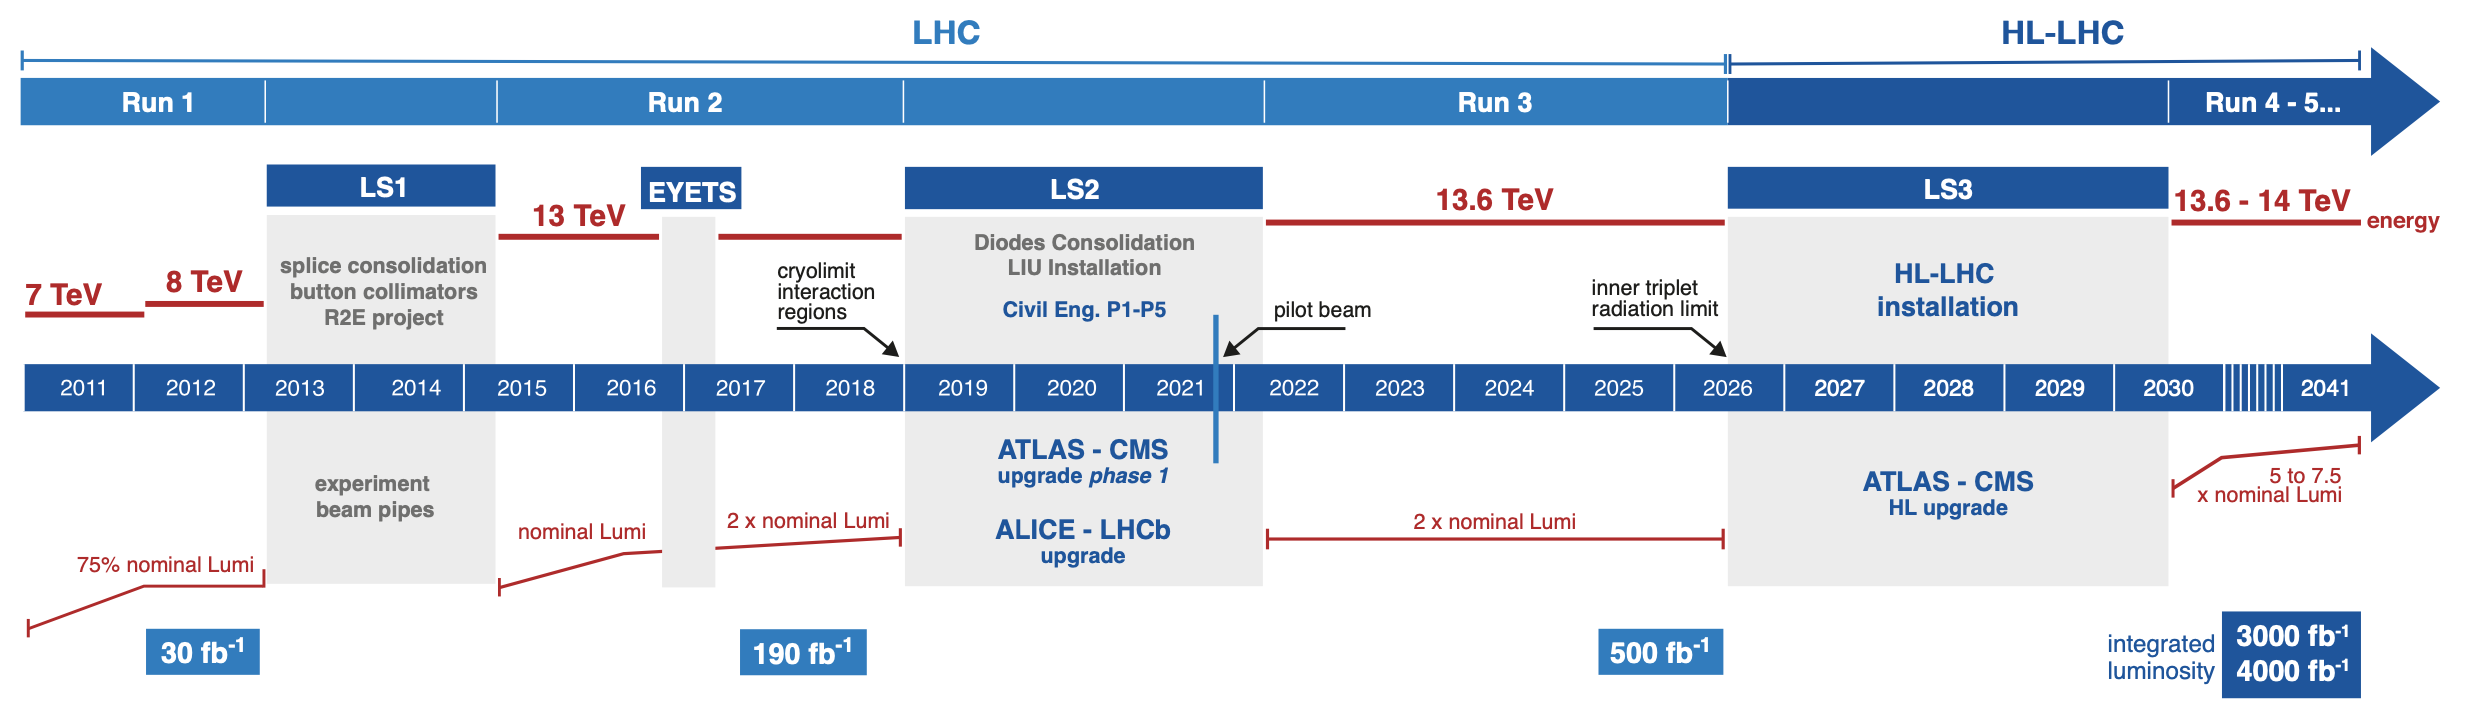
\includegraphics[width=\linewidth]{fig/lhc_hl_lhc.png}
\caption[Current and future timeline of LHC operations as of 2025 with corresponding center-of-mass energies and projected integrated luminosities.]{\label{fig:lhc:hl_lhc}Current and future timeline of \acs{LHC} operations with corresponding center-of-mass energies and projected integrated luminosities. \citep{lhc:hl_lhc}.}
\end{center}
\end{figure}
%\end{wrapfigure}

Operations at the \acs{LHC} are defined in periods of data-taking and shut-down known as runs and long shutdowns respectively; the first period (Run 1) started with first collisions at the \acs{LHC} in 2010 at $\acs{Ecom}=7$ TeV \citep{PERF-2010-01}. Upgrades are usually carried out for detectors and accelerators during long shutdowns, raising the maximum energy threshold in preparation for the next run. An overview of the \acs{LHC} runtime and corresponding center-of-mass energies are summarized in \autoref{fig:lhc:hl_lhc}. During Run 2 from 2015-2018, the \acs{ATLAS} detector recorded a total of $1.1\times 10^{16}$ \acs{pp} collisions at $\acs{Ecom}=13$ TeV, which corresponds to an integrated luminosity of $140 \pm 0.83\%$ \fb that passed data quality control and are usable for analyses \citep{DAPR-2021-01}. This is also the data set used for the analysis in this dissertation.

\textcolor{red}{status/plan for run 3 and beyond?}

\subsection{Physics at the LHC}
The majority of physics studied at the \acs{LHC} focus primarily on \acs{QCD} proton-proton hard scattering processes and the resulting products. Hard scattering processes involve large momentum transfer compared to the proton mass e.g. top pair production ($gg\rightarrow\ttbar$) and Higgs production ($gg\rightarrow H$), and can be predicted using perturbative \acs{QCD} \citep{theory:hard_process}. Hard processes probe distance scales much lower than the proton radius and can be considered collisions between the constituent quarks and gluons i.e. partons. Soft processes involve lower momentum transfer between partons and are dominated by less well-understood non-perturbative \acs{QCD} effects. The hard interaction between two partons are represented by a parton distribution function (\acs{PDF}) $f_i(x, Q^2)$, which describes the probability of interacting with a constituent parton $i$ that carries a fraction $x$ of the external hadron's momentum when probed at a momentum scale of $Q^2$ \citep{theory:hard_process2}. Other partons within the hadron that did not participate in the collision can still interact via lower momentum underlying-events (\acs{UE}). The probability of a particular interaction occurring is defined as its cross-section \acs{xsec}. \autoref{fig:lhc:xsec} gives an overview of \acs{SM} processes produced within the \acs{LHC} and their cross-sections. 
%Interactions at the \acs{LHC} are dominated by top pair-production from gluon fusion $gg \rightarrow \ttbar$ (85\%)

\begin{figure}[!htb]
\begin{center}
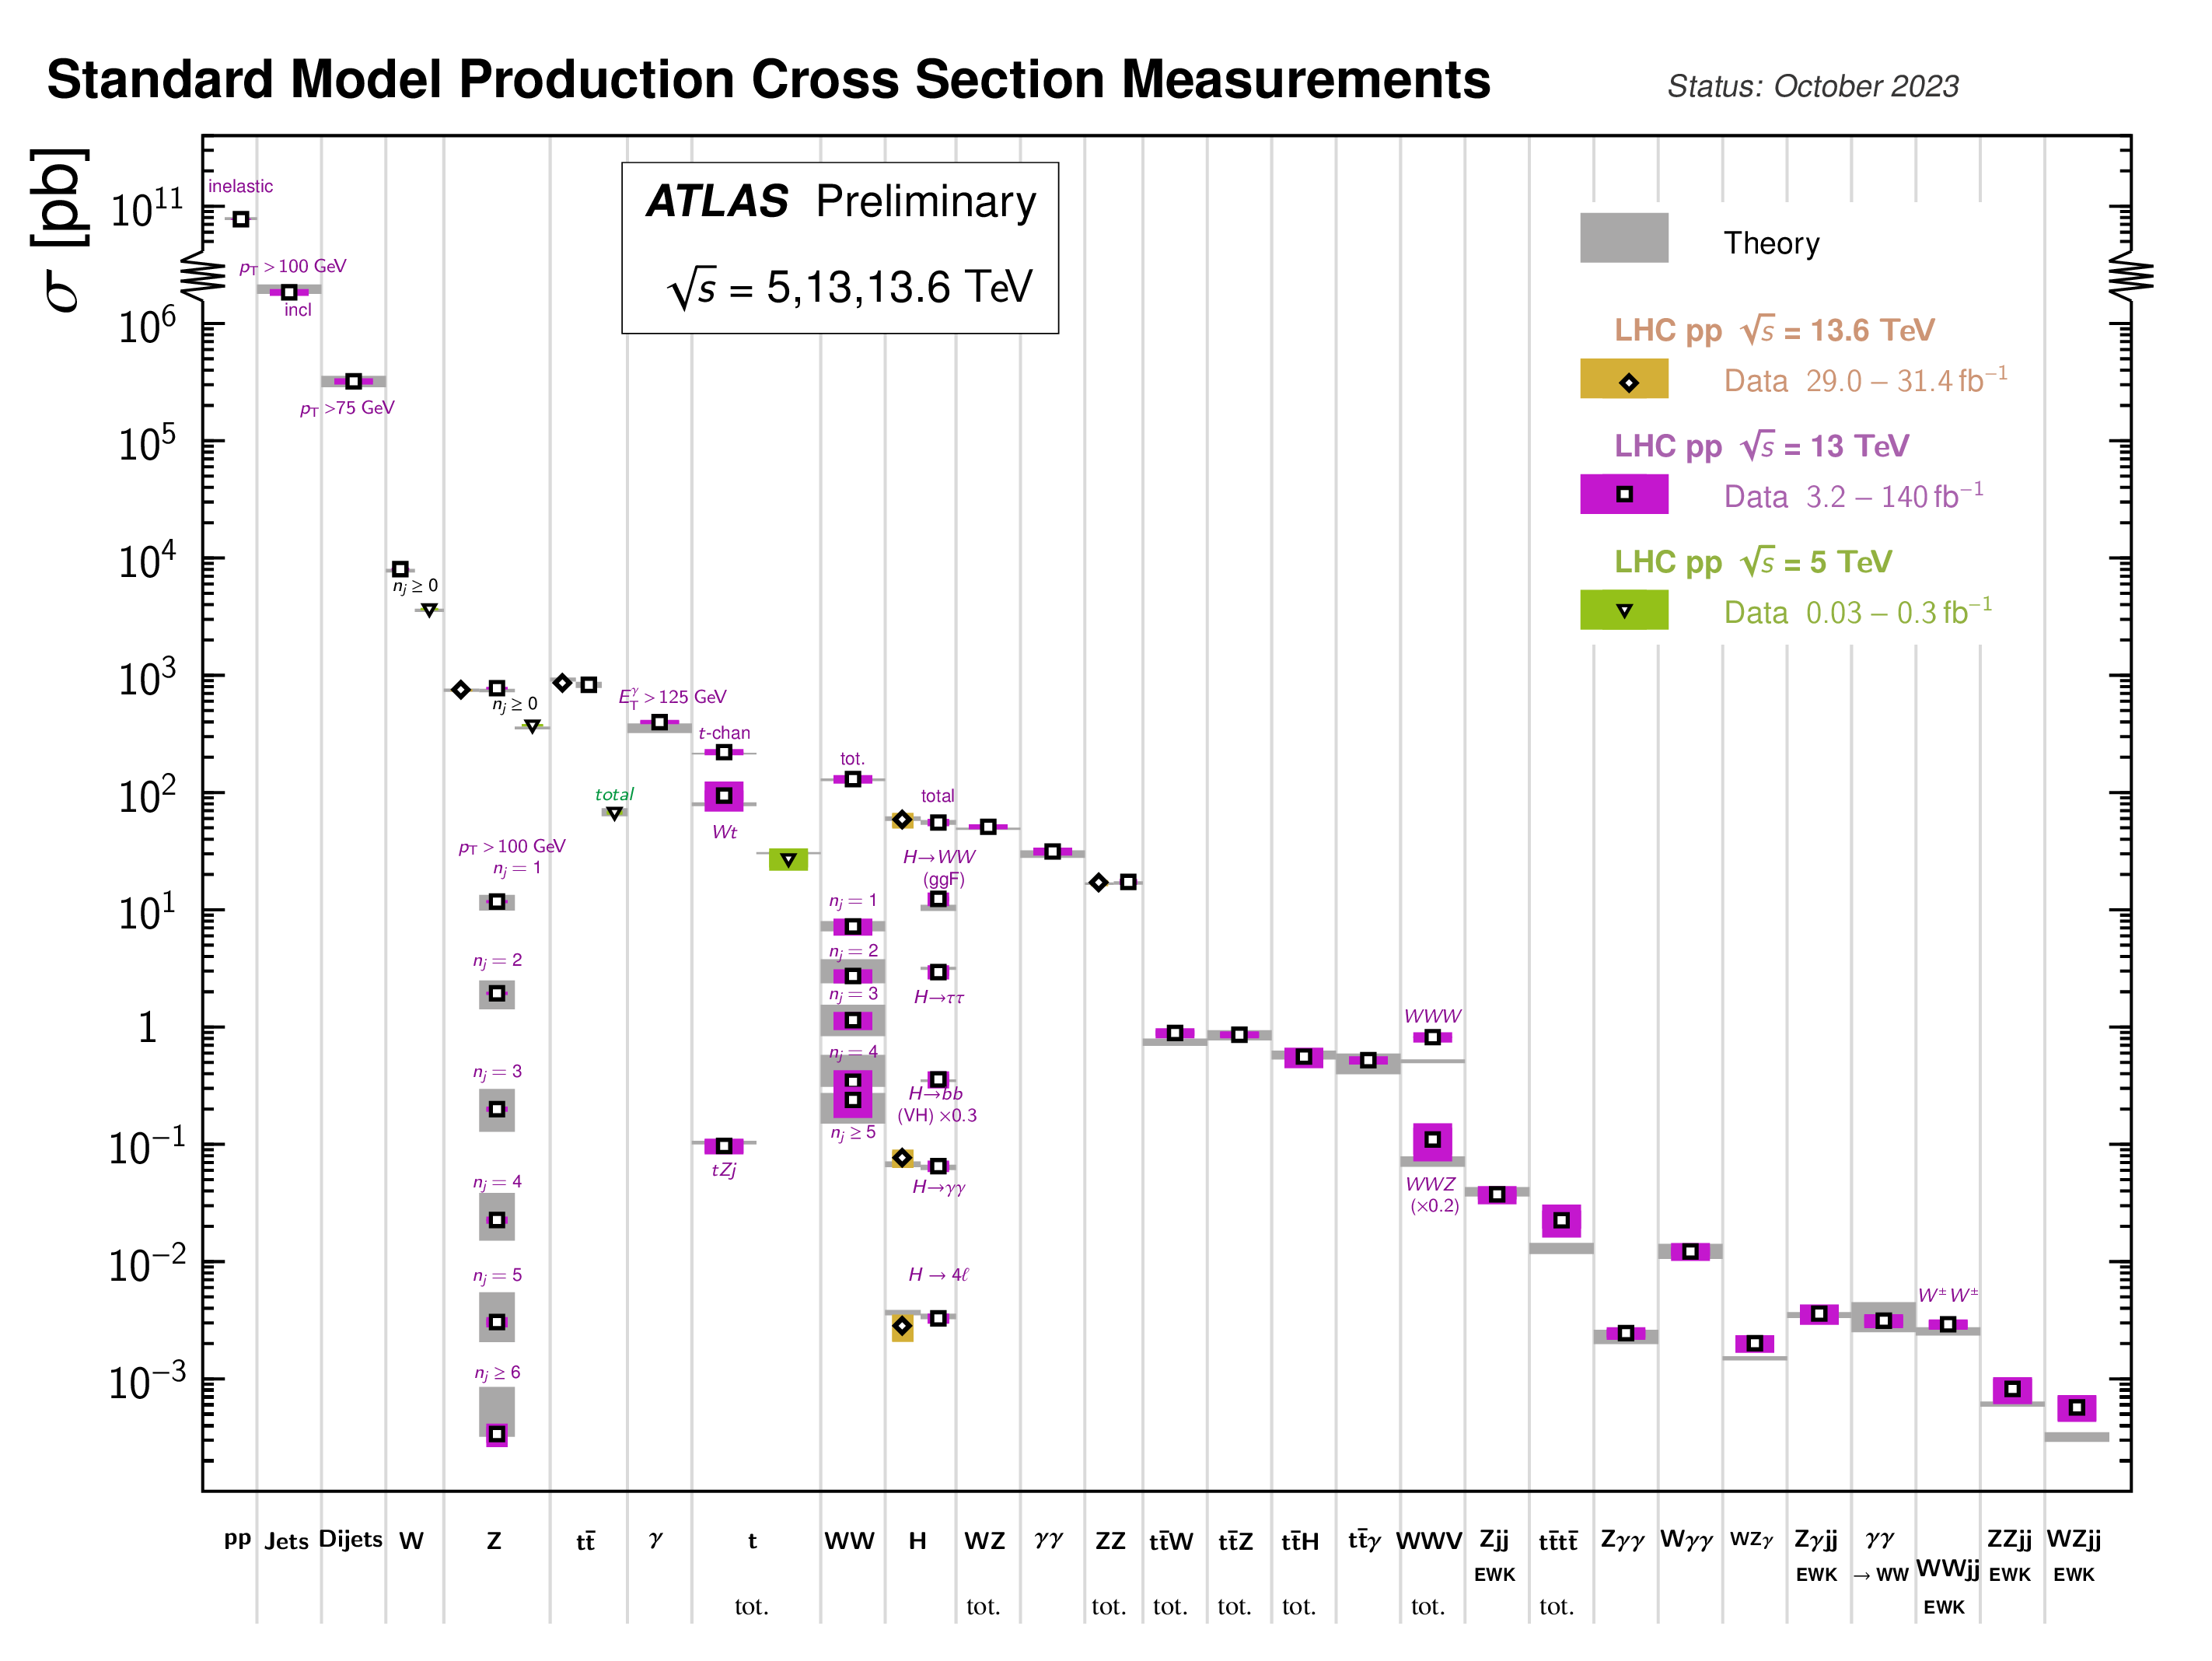
\includegraphics[width=\linewidth]{fig/lhc_xsec_Run23.png}
\caption[Summary of predicted and measured cross-section for SM processes at the LHC at different center-of-mass energies]{\label{fig:lhc:xsec}Summary of predicted and measured cross-section for \acs{SM} processes at the \acs{LHC} at different center-of-mass energies \citep{ATL-PHYS-PUB-2023-039}.}
\end{center}
\end{figure}

\section{The ATLAS detector}
\label{sec:ATLAS}

One of the four main experiments at the \acs{LHC} is \acs{ATLAS} \citep{atlas}, designed as a multi-purpose detector for the role of studying high-energy physics in \acs{pp} and heavy-ion collisions. \acs{ATLAS} is a detector with symmetric cylindrical geometry with dimensions of 44 m in length and 25 m in diameter, covering a solid angle of almost $4\pi$ around the collision point. The detector is built concentrically around the beamline with the collision point at the center to maximally capture signals produced by interactions. \autoref{fig:lhc:atlas} shows a slice of the ATLAS detector. From the inside out, the main \acs{ATLAS} subdetector system consists of the inner detector (\acs{ID}), calorimeter systems (electromagnetic and hadronic) and the muon spectrometer (\acs{MS}).

\begin{figure}[!htb]
\begin{center}
%\subfloat[]{
%\includegraphics[width=0.5\linewidth]{fig/lhc_atlas_schematics.png}}
%\subfloat[]{
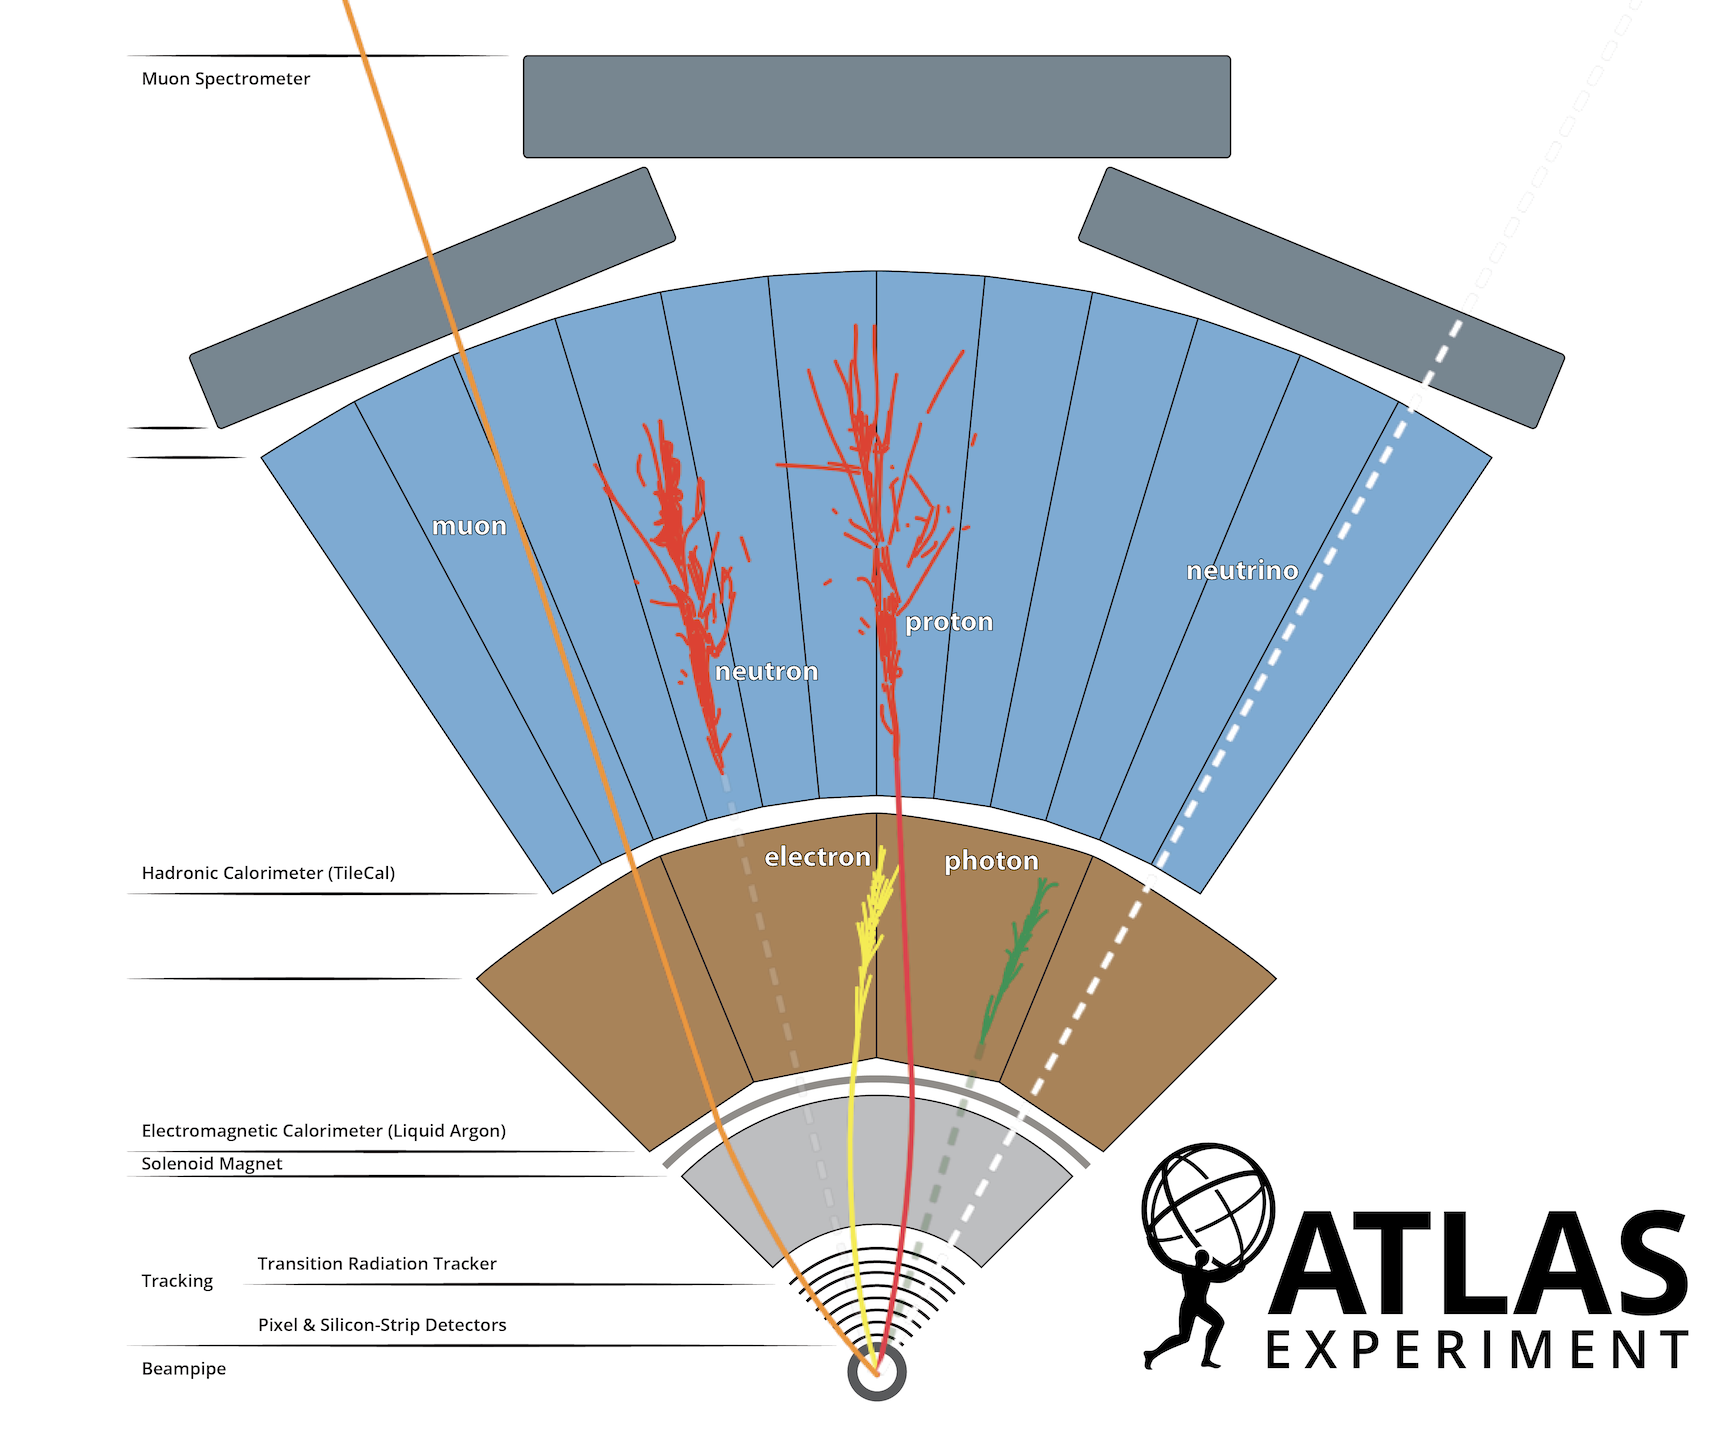
\includegraphics[width=\linewidth]{fig/lhc_atlas_particle_path_white.png}
%}
\caption[A cross section slice of the ATLAS detector showing different subsystems along with visualization of different types of particles traveling through the detector]{\label{fig:lhc:atlas}A cross section slice of the \acs{ATLAS} detector showing different subsystems along with visualization of different types of particles traveling through the detector \citep{lhc:atlas_detector}.}
\end{center}
\end{figure}

The \acs{ATLAS} detector uses a right-handed coordinate system \citep{atlas} designed to align with the geometry of a collision interaction, with the origin set at the interaction point, the $z$-axis following (either of) the beamline and the $x$-axis pointing towards the center of the \acs{LHC} ring. In cylindrical coordinates, the polar angle $\theta$ is measured from the beam axis, and the azimuthal angle $\phi$ is measured along the transverse plane ($xy$-plane) starting at the $x$-axis. Addtional observables are defined for physics purposes: the pseudorapidity defined as $\acs{eta} = -\ln \tan (\theta/2)$; angular distance within the detector defined as $\acs{dR} = \sqrt{\Delta \acs{eta}^2 + \Delta\phi^2}$; and transverse momentum \acs{pT} (transverse energy \acs{ET}) defined as the component of the particle's momentum (energy) projected onto the transverse plane. 
%The detector is further divided into barrel ($1\lesssim \acs{eta}|\lesssim 1.4$) and endcap regions ($1.4 \lesssim |\acs{eta}| \lesssim 3.2$) for coverage of particles traveling closer to the transverse plane and the beam axis respectively.

\subsection{Inner detector}
The innermost part of \acs{ATLAS} is the inner detector (\acs{ID}) \citep{atlas}, constructed primarily for the purpose of measuring and reconstructing charged tracks within the $|\acs{eta}|<2.5$ region with high momentum resolution ($\sigma_{\pT} / \pT = 0.05\% \pm 1\%$). \autoref{fig:lhc:atlas_id} shows the composition of the \acs{ID} with three subsystems, the innermost being the pixel detector, then Semiconductor Tracker (\acs{SCT}), and the Transition Radiation Tracker (\acs{TRT}) on the outermost layer; all of which are surrounded by a solenoid magnet providing a magnetic field of 2 T.

\begin{figure}[!htb]
\begin{center}
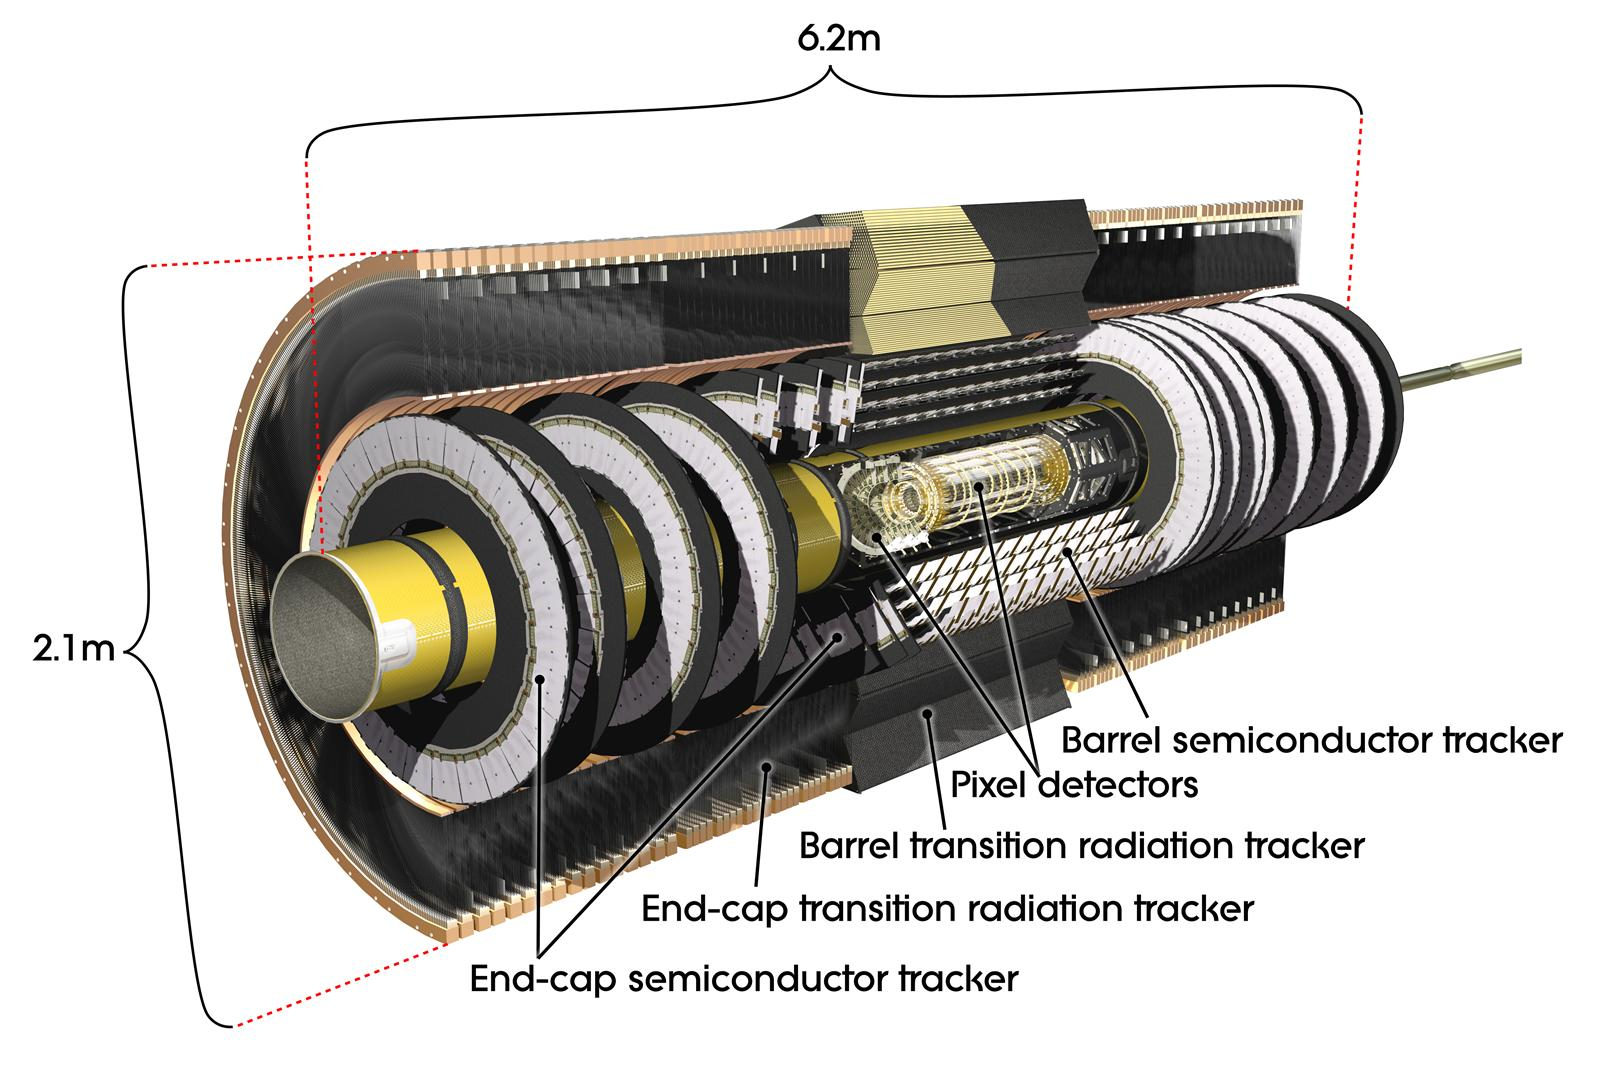
\includegraphics[width=0.7\linewidth]{fig/lhc_atlas_id.jpg}
\caption[Cutaway illustration of the inner detector along with its subsystems.]{\label{fig:lhc:atlas_id}Cutaway illustration of the inner detector along with its subsystems \citep{lhc:atlas_id}.}
\end{center}
\end{figure}

\subsubsection*{Pixel detector}
The pixel detector subsystem \citep{atlas} consists of 250 \textmu m silicon semiconductor pixel layers with about 80.4 million readout channels, reaching a spatial resolution of 10 \textmu m in the $R-\phi$ (transverse) plane and 115 \textmu m in the $z$-direction for charged tracks. Charged particles passing through the pixel detector ionize the silicon layers and produce electron-hole pairs; the electrons drift towards the detector's electrode under an applied electric field and the resulting electric signals are collected in read-out regions. The pixel detector is used primarily for impact parameter measurement, pile-up suppression, vertex finding and seeding for track reconstruction.

\subsubsection*{Semiconductor Tracker}
The Semiconductor Tracker (\acs{SCT}) \citep{atlas} functions similarly to the pixel detector, using silicon semiconductor microstrips totaling about 6.3 million read-out channels, reaching a per layer resolution of 17 \textmu m in the $R$-$\phi$ plane and 580 \textmu m in the $z$-direction \citep{atlas}. The \acs{SCT} plays an important role in precise \pT measurement of charged particles as well as track reconstruction.

\subsubsection*{Transition Radiation Tracker}
The outermost layer of the \acs{ID}, the Transition Radiation Tracker (\acs{TRT}) \citep{atlas}, consists of layers of 4 mm diameter straw tubes filled with a xenon-based gas mixture and a 30 \textmu m gold-plated wire in the center. The \acs{TRT} contains a total of about 351 thousand readout channels with a resolution of 130 \textmu m for each straw tube in the $R$-$\phi$ plane, and provides extended track measurement, particularly estimation of track curvature under the solenoidal magnetic field. Importantly, the \acs{TRT} also serves to identify electrons through absorption of emitted transition-radiation within the Xe-based gas mixture.


\subsection{Calorimeter systems}
Surrounding the \acs{ID} is the ATLAS calorimeter system \citep{atlas} with electromagnetic (\acs{EM}) and hadronic calorimeters, covering a range of $|\acs{eta}|<4.9$. The calorimeters are sampling calorimeters with alternating absorbing layers to stop incoming particles and active layers to collect read-out signals from energy deposits. Incoming particles passing through the calorimeters interact with the absorbing layers, producing \acs{EM} or hadronic showers of secondary particles. The particle showers deposit energy in the corresponding layer of the calorimeters, which are collected and aggregated to identify and reconstruct the original particle's energy and direction. \autoref{fig:lhc:atlas_calo} shows a schematic overview of the ATLAS calorimeter system.

\begin{figure}[!htb]
\begin{center}
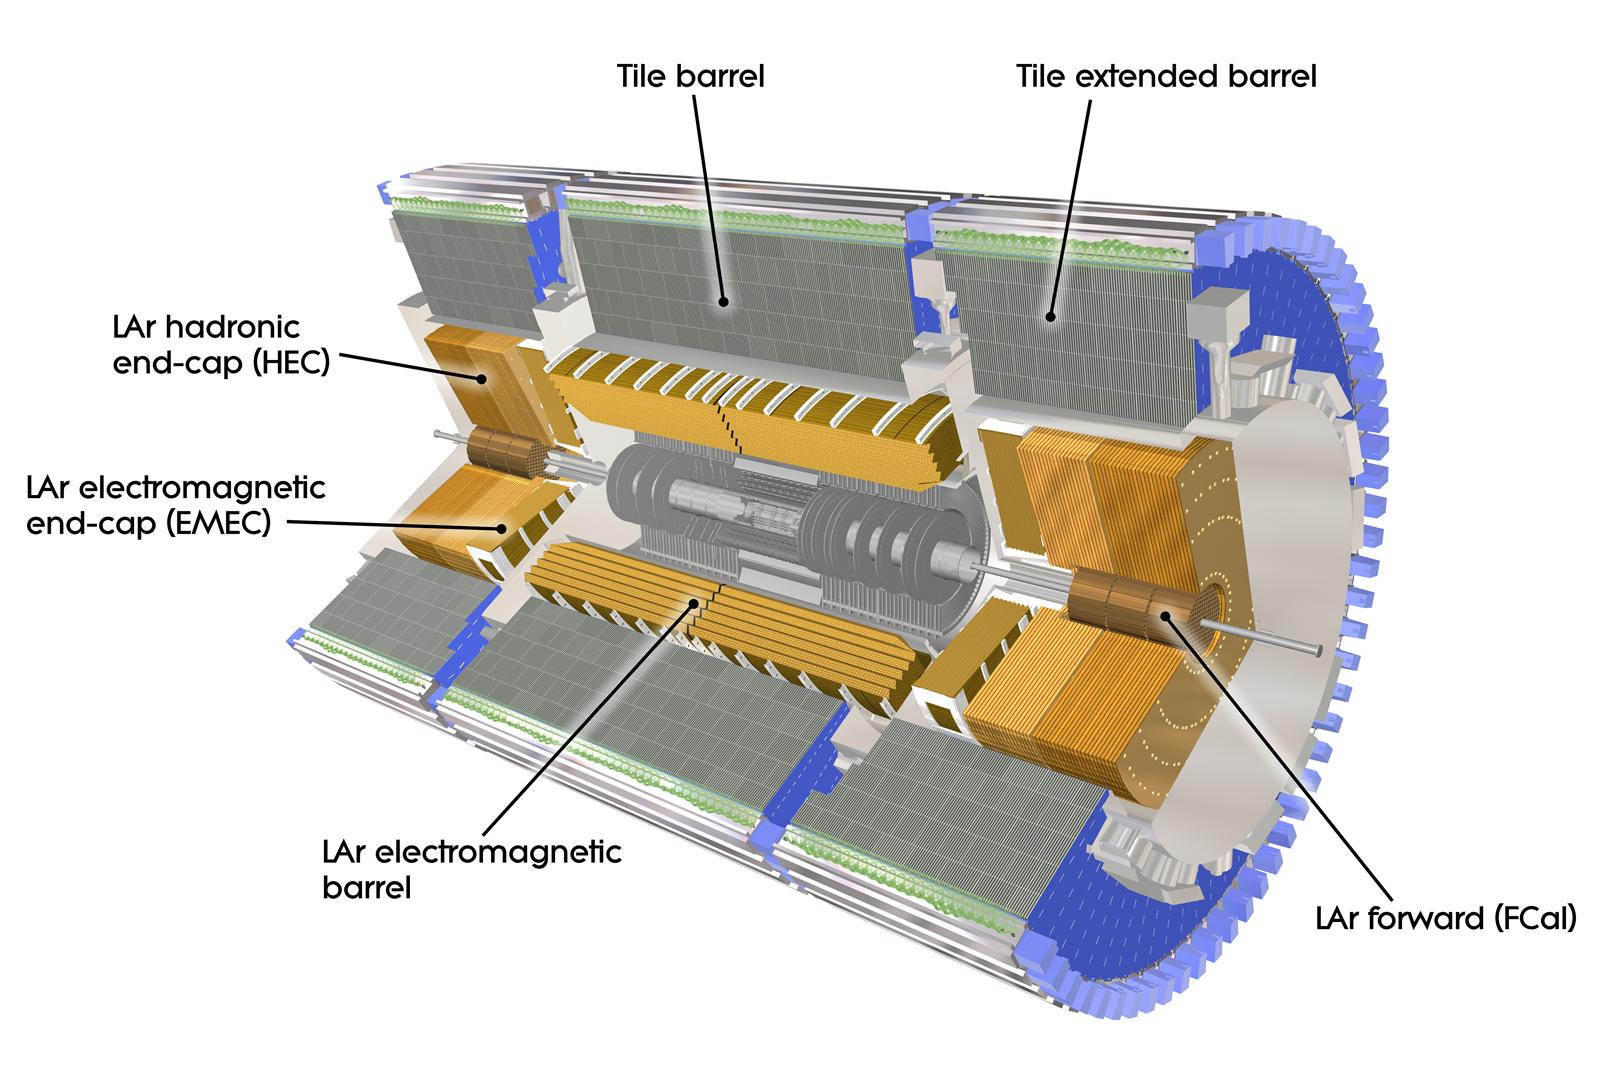
\includegraphics[width=0.7\linewidth]{fig/lhc_atlas_calorimeter.jpg}
\caption[Cutaway illustration of the calorimeter system including the \acs{EM}, hadronic and \acs{LAr} forward calorimeters ]{\label{fig:lhc:atlas_calo}Cutaway illustration of the calorimeter system including the \acs{EM}, hadronic and \acs{LAr} forward calorimeters \citep{lhc:atlas_calo}.}
\end{center}
\end{figure}

\subsubsection*{Electromagnetic calorimeter} 
The \acs{EM} calorimeter \citep{atlas} covers the innermost part of the calorimeter system, with lead (Pb) absorbing layers and liquid argon (\acs{LAr}) active layers to capture the majority of electrons and photons exiting the \acs{ID}. The \acs{EM} calorimeter is divided into regions depending on \acs{eta} coverage: a barrel region ($|\acs{eta}|<1.475$), two endcap regions ($1.375<|\acs{eta}|<3.2$) and a transition region ($1.372<|\acs{eta}|<1.52$). The endcap calorimeters are further divided into an outer wheel region ($1.372<|\acs{eta}|<2.5$) and an inner wheel region ($2.5<|\acs{eta}|<3.2$) in order to provide precise coverage within the same \acs{eta} range as the \acs{ID}. Overlap between the barrel and endcap regions compensates for the lower material density in the transition region.

%\columnbreak
\subsubsection*{Hadronic calorimeter}
The hadronic calorimeter \citep{atlas} covers up to $|\acs{eta}|<4.9$ and is comprised of three parts: the tile calorimeter with a barrel region ($|\acs{eta}|<1.0$) and extended barrel regions ($0.8<|\acs{eta}|<1.7$); the hadronic endcap calorimeter (\acs{HEC}) covering $1.5<|\acs{eta}|<3.2$; and the forward calorimeter (\acs{FCal}) covering $3.2<|\acs{eta}|<4.9$. The tile calorimeter covers the \acs{EM} calorimeter barrel region and uses steel as material for the absorbing layers with scintillating tiles for the active layers. Signals captured by scintillating tiles are read out from both sides using photomultiplier tubes. The \acs{HEC} calorimeter covers the endcap regions of the \acs{EM} calorimeter and uses a copper-\acs{LAr} calorimeter layer scheme. The \acs{FCal} is located close to the beamline providing coverage for particles traveling close to parallel with the beam axis. The subdetector contains three modules: one with copper absorbing layers optimized for \acs{EM} measurements, and two with tungsten absorbing layers targeting hadronic cascades. All modules in the \acs{FCal} use \acs{LAr} as the active layer.

\subsection{Muon spectrometer}
Generally, the only particles that penetrate past the calorimeter layer are muons and neutrinos. The muon spectrometer (\acs{MS}) \citep{atlas} is situated on the outermost of the ATLAS detector and aims to track and measure muons within $|\acs{eta}|<2.7$.The \acs{MS} utilizes an array of toroid magnets to provide a magnetic field perpendicular to the muon trajectory, bending the track in order to measure its curvature. The magnetic field is powered by a large barrel toroid ($|\acs{eta}|<1.4$) with strength of 0.5 T and two endcap toroid magnets ($1.6<|\acs{eta}|<2.7$) of 1 T. Both types contribute to the magnetic field in the transition region ($1.4<|\acs{eta}|<1.6$).

To measure the muon itself, four types of large gas-filled chambers known as muon chambers \citep{atlas} are designed and constructed for two main goals: triggering on potential muon candidates entering the \acs{MS} and tracking their trajectories through the detector with high precision. The tracking system include Monitored Drift Tubes (\acs{MDT}s), which record muon track information over the entire \acs{MS} \acs{eta} range ($|\acs{eta}|<2.7$). The \acs{MDT}s are built with multiple layers of drift tubes and filled with a mixture of 93\% Ar and 7\% $\text{CO}_2$.  Muons passing through drift tubes in the \acs{MDT} ionize the gas within each tube; signals are then recorded as freed electrons drift to read-out channels under an applied electric field. In the forward region ($2.0<|\acs{eta}|<2.7$), Cathode Strip Chambers (\acs{CSC}s) are included along with \acs{MDT}s. The \acs{CSC}s are multiwire proportional chambers built with higher granularity and shorter drift time than the \acs{MDT}s to handle tracking in an environment with high background rates .

The \acs{MS} trigger system includes Resistive Plate Chambers (\acs{RPC}s) \citep{atlas}, which provide triggering in the barrel region ($|\acs{eta}|<1.05$) using parallel electrode plates made of resistive materials with a gas mixture inbetween. High voltage is applied to the plates, accelerating the electrons freed from ionized gas and creating a fast avalanche of charge, which is collected on external read-out strips almost instantaneously. Triggering and coarse position measurements in the endcap region ($1.05<|\acs{eta}|<2.5$) is handled by Thin-Gap Chambers (\acs{TGC}s). Similar to \acs{CSC}s, \acs{TGC}s are multiwire proportional chambers with a small wire gap ("thin-gap") and high applied voltage across the gap, resulting in fast response time giving \acs{TGC}s the capabilities to identify muon candidates in real time.
	
%\subsection{Forward detectors}
%\begin{itemize}
%\item LUCID (LUminosity measurement using Cherenkov Integrating Detector): $\pm 17$ m from interaction point, measures luminosity using $pp$ scattering in the forward region
%\item ALFA (Absolute Luminosity for ATLAS): $\pm 240$ m, measures $pp$ scattering at small angles
%\item ZDC (Zero-Degree Calorimeter): $\pm 140$ m, measures centrality in heavy-ion collisions
%\end{itemize}

%\subsection{Magnetic systems}
%superconducting solenoid \& toroid magnets cooled to 4.5 K with liquid helium\\
%solenoid: 2.56 m diameter, 5.8 m length, 2 T strength axial magnetic field, encloses inner detector\\
%toroid = barrel + endcap toroid x2\\
%barrel toroid: 9.2/20.1 m inner/outer diameter, 25.3 m length, 0.5 T strength\\
%endcap toroid: 1.65/10.7 m inner/outer diameter, 5 m length, 1 T strength\\
%(show magnet system diagram)

\subsection{Trigger \& data acquisition}
The \acs{LHC} produces a colossal amount of collision data at a bunch crossing rate of 40 MHz with bunch spacing of 25 ns. The ATLAS Trigger and Data Acquisition (\acs{TDAQ}) system \citep{lhc:atlas_trigger} synchronously identifies and records interesting events for in-depth analysis. The ATLAS trigger system in Run 2 consists of two steps: Level-1 (\acs{L1}) trigger and High-Level Trigger (\acs{HLT}). Events failing any step in the trigger chain are permanently lost.

The \acs{L1} trigger hardware is divided into \acs{L1} calorimeter triggers (L1Calo) and \acs{L1} muon triggers (L1Muon) \citep{lhc:atlas_trigger}. L1Calo trigger uses information from ATLAS calorimeter system to quickly identify signs of high \pT objects e.g. \acs{EM} clusters, jets and missing transverse energy \acs{ETmiss} (\autoref{sec:met}). Similarly, L1Muon uses information from the \acs{RPC}s and \acs{TGC}s of the \acs{MS} to make quick decisions on potentially interesting muon candidates. Outputs from L1Calo and L1Muon are fed into the \acs{L1} topological trigger (L1Topo) for additional filtering based on event topology and multi-object correlation, allowing for more selective and physics-motivated triggering. Decisions from all three types of \acs{L1} triggers are provided as inputs for the Central Trigger Processor (\acs{CTP}) for a final Level-1 Accept (L1A) decision. The entire \acs{L1} trigger chain results in a 2.5 \textmu s latency and reduces the event rate to 100 kHz.

Events passing \acs{L1} triggers are sent to \acs{HLT}s before being saved to offline storage at \acs{CERN} data centers. \acs{HLT}s are software-based triggers used for more complex and specific selections on physics objects required by targeted analysis goals, in turn requiring more computing power with longer latency. After \acs{HLT} selections, the event rate is reduced to 1 kHz on average  \citep{lhc:atlas_trigger}. Overall, the full trigger chain reduces the event rate for ATLAS by approximately a factor of $4\times 10^4$.
\end{document}